Section~\ref{sec:collapse} measured a four-order-of-magnitude rise in
$\kappa(\bar H)$ and a ten-fold rise in the interpolator's norm. This section
derives both from one assumption, that each adapter's $A$ factor is a small
displacement of a common start. It then tests the derivation against the
adapters, and tests a scalar law derived from it on training regimes it was
not calibrated on.

\paragraph{Set-up.} In a shared cohort, $A_t = A_0 + E_t$. Let
$W_0 \in \R^{d\times r}$ be an orthonormal basis of the row space of $A_0$ and
$P_\perp = I - W_0 W_0^\top$. Whenever $W_0^\top A_t^\top$ is invertible, the
row space $V_t$ of $A_t$ is exactly the graph of a \emph{tilt}
\begin{equation}\label{eq:tilt}
  X_t \;=\; P_\perp A_t^\top \bigl(W_0^\top A_t^\top\bigr)^{-1} \in \R^{d\times r},
  \qquad V_t = \operatorname{col}(W_0 + X_t),
\end{equation}
and the principal angles between $V_t$ and the starting subspace satisfy
$\tan\theta_i = \sigma_i(X_t)$. The tilt is of the order of the relative
displacement:
\[
  \|X_t\| \;\lesssim\; \|E_t\| / \sigma_{\min}(A_0).
\]
Write
$D_t = \Delta W_t$ for the task updates and $M_t = D_t(W_0 + X_t)$ for their
action on the tilted bases.

\begin{proposition}[First-order conditioning of a shared cohort]
\label{prop:drift}
Let $Y = [X_1 - \bar X, \dots, X_T - \bar X] \in \R^{d\times Tr}$ collect the
centred tilts and $\Sigma_X = \tfrac1T Y Y^\top$. To leading order in the tilt,
\begin{enumerate}[leftmargin=*,itemsep=1pt,topsep=2pt]
\item $\bar H$ has $r$ eigenvalues $1 - O(\|X\|^2)$ and $(T-1)r$ eigenvalues
  equal to the nonzero eigenvalues of $\Sigma_X$, so
  $\kappa(\bar H) \approx 1/\lambda_{\min}^{+}(\Sigma_X)$;
\item the exact interpolator is $\tauH \approx a\,W_0^\top + b$ with
  $b = [M_1 - \bar M, \dots, M_T - \bar M]\, Y^{+}$ and $a = \bar M - b\bar X$;
\item under a uniform rescaling of the displacements $E_t \mapsto sE_t$,
  $\kappa(\bar H) \propto s^{-2}$ while the amplification
  $\|\tauH\|/\|\bar D\| \propto s^{-1}$.
\end{enumerate}
\end{proposition}

The derivation, in Appendix~\ref{app:theory}, expands each projector to second
order in $X_t$ and takes the Schur complement of $\bar H$ on the orthogonal
complement of the starting subspace. The interpolation conditions
$\tauH(W_0 + X_t) = M_t$ then separate into a component along $W_0$ and one
along the centred tilts. In words: the subspaces share $r$ directions almost
exactly, those directions are well conditioned, and everything else a merge
must resolve lives in the small differences between the tilts.
Figure~\ref{fig:theory}a shows this on a real layer: the prediction follows
the exact spectrum of $\bar H$ across all $48$ small eigenvalues, not only at
the smallest one that sets $\kappa$.

\paragraph{A consequence.} The amplification is of first order in the inverse
displacement and $\kappa$ of second order. And $\kappa(\bar H)$ is set by the
\emph{smallest} singular value of the spread of the displacements, not by
their size. A displacement of $13\%$ in every direction would give
$\kappa \approx 60$. The measured $10^{4}$ to $10^{5}$ therefore means that
training displaces the adapters very unevenly, leaving some directions of the
spread almost unexcited. On synthetic cohorts the same relative displacement
gives $\kappa \approx 5\times10^{2}$ with isotropic displacements and $10^{5}$
to $10^{6}$ with low-rank ones (Appendix~\ref{app:theory}).

\paragraph{Tests.} We registered five predictions before computing any of the
quantities involved, and all five hold (Figure~\ref{fig:theory}).
\begin{itemize}[leftmargin=*,itemsep=1pt,topsep=2pt]
\item \emph{The conditioning, during training.} On a Llama-3.1-8B cohort whose
  $A_0$ was saved before the first optimiser step, the first-order prediction
  of $\kappa(\bar H)$ equals the exact value at $25$, $50$, $75$ and $100\%$
  of training.
\item \emph{The amplification, during training.} The same holds for the
  amplification on the same cohort and checkpoints.
\item \emph{The formula, without $A_0$.} A reference-free version, which takes
  the consensus subspace of the cohort as $W_0$ and needs no saved start, does
  the same on all twelve shared cohorts of the four bases, and on the five
  task-count and rank configurations of \S\ref{subsec:tr}.
\item \emph{The orders.} Rescaling the measured displacements by five factors
  $s$ from $0.05$ to $1$ gives exact log-log slopes of $-2.00$ for
  $\kappa$ and $-1.01$ for the amplification, inside the registered bands
  $[-2.2, -1.8]$ and $[-1.2, -0.8]$. The rival $s^{-2}$ form for the
  amplification is excluded.
\item \emph{Across training.} Both quantities fall monotonically as the
  adapters drift, $\kappa$ from $2.7\times10^{4}$ to $1.1\times10^{4}$ and the
  amplification from $61$ to $44$.
\end{itemize}
Across the $21$ configurations, the predicted $\kappa(\bar H)$ lies between
$0.9990$ and $1.0005$ times the exact value, within $0.10\%$. The predicted
amplification matches to six digits, but that match is close to algebraic and
we do not count it as evidence: the interpolation conditions behind item~2 of
the proposition are exact, and the one approximation, dropping a coupling
through $\bar X$, vanishes for the consensus $W_0$ of the reference-free test.
The evidence for the expansion is the agreement of $\kappa$, which rests on the
second-order expansion of the projectors, and the two slopes.

\paragraph{Out of sample.} These tests compute each prediction from the same
adapters' tilts. A stronger test is whether the scaling of item~3 carries to
cohorts trained differently. Item~3 implies a scalar law,
$\kappa(\bar H) \approx C_\kappa / t^2$ and amplification $\approx C_a / t$,
where $t$ is the median over tasks and layers of the spectral norm of the tilt
$X_t$ under the consensus $W_0$. We fixed $C_\kappa$ and $C_a$ on the four
existing shared Llama-3.1-8B cohorts and committed them before training the
seven cohorts of \S\ref{subsec:tr} (learning rate, epochs, $A$'s learning
rate, LoRA+ and the scale of $A_0$), which with the baseline cohort trained
alongside them give eight test cohorts. The registered thresholds were a
factor of $2$ for $\kappa$ on at least six and a factor of $1.25$ for the
amplification on at least seven. The law predicts $\kappa$ within a factor of
$2$ on all eight, over a range from $1.2\times10^{3}$ to $5.5\times10^{4}$,
and the amplification within $1.25$ on seven. Across the eight cohorts $t$ and
$\kappa$ have Spearman correlation $-0.976$. Reaching the independent arm's
median $\kappa$ of $1.55$ would take a tilt of $t^\star = 22$, $27$ times the
largest tilt any regime produced ($0.83$). The shared cohorts trained at three
times the learning rate and at four times $A$'s learning rate leave
adapter-only RegMean at $\lambda = 10^{-6}$ with an excess of $0.34$ and
$0.38$ nats, against $0.057$ and $0.073$ for their independent counterparts.
All five predictions of this second registration hold, and it permits saying
that the scalar law predicts $\kappa$ on these regimes. That claim is limited
to one base model and to changes of training that keep a shared start.

One regime departs from the picture in a way we did not predict. Scaling
$A_0$ by $0.25$ before training gives the largest relative tilt ($0.83$),
$\kappa(\bar H) = 1.2\times10^{3}$, and an amplification of $7.5$, about half
the $13.7$ the law predicts; it is the one amplification miss. On this cohort
adapter-only RegMean at $\lambda = 10^{-6}$ leaves an excess of only $0.022$
nats, below the independent cohort's $0.071$. Three times the learning rate
reaches the same $\kappa$ ($1.2\times10^{3}$) with an amplification of
$15.9$, and there the excess is $0.34$. The two cohorts have equal $\kappa$
and differ in amplification, and the solver's damage differs with it. We note
this as an observation from two cohorts; a smaller initial $A$ as a mitigation
would need its own test.

\begin{figure}[pos=tbp]
\centering
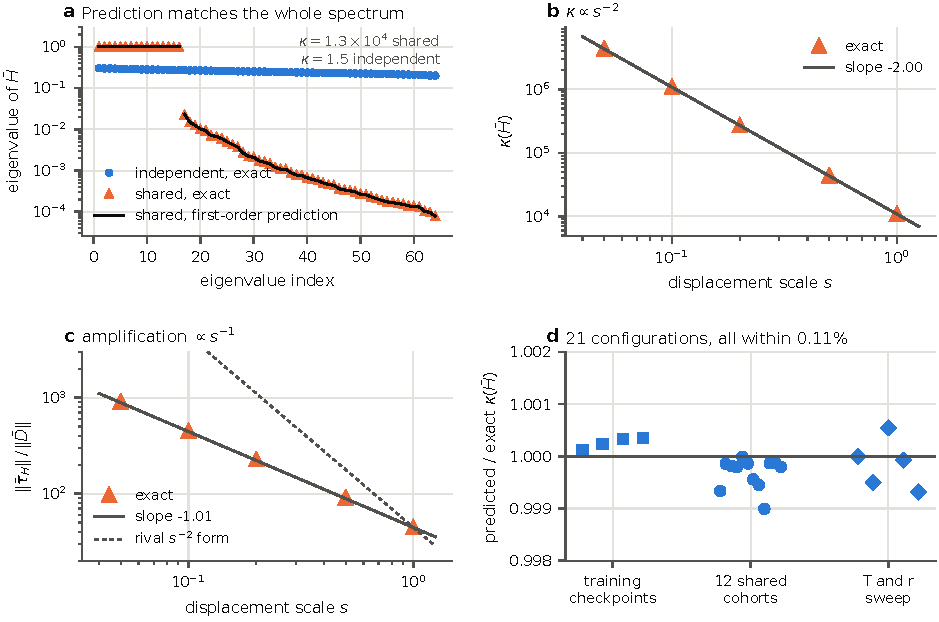
\includegraphics[width=\textwidth]{nc/figures/fig2_theory.pdf}
\caption{The first-order theory against exact values. \textbf{(a)} All $64$
eigenvalues of $\bar H$ for one layer of a Llama-3.1-8B cohort (the layer with
the median $\kappa$ of the eight sampled): on the shared cohort, $r = 16$
eigenvalues sit at $1$ and the other $48$ follow the eigenvalues of
$\Sigma_X$ that Proposition~\ref{prop:drift} predicts (line); on the
independent cohort all $64$ sit near $1/T$. \textbf{(b, c)} The displacements
of a shared cohort rescaled by $s$; lines have the fitted slopes, and the dashed
line in (c) is the rival $s^{-2}$ form, which the data exclude.
\textbf{(d)} Predicted over exact $\kappa(\bar H)$ at four training
checkpoints, on twelve shared cohorts of four bases, and at five task counts
and ranks. All $21$ ratios lie in $[0.9990, 1.0005]$.}
\label{fig:theory}
\end{figure}

\paragraph{Scope.} The proposition is a leading-order expansion
checked numerically, not a bound with explicit constants. It describes the
shared regime only; in the independent regime the tilts are not small and the
amplification equals $T$ by a separate identity. It explains the
conditioning a solver would face, and its scalar form predicts that
conditioning across the training regimes we tested; whether a given solver
faces it is the question of \S\ref{sec:merging}.
